

This section covers a description of the robot, along with potential consderations for alternatives wihtin each decision.
\subsection{Mechanics}
During the design proces of the project it was identified that the main obstacle would be friction. As such many design choices came down to minimizing that factor. 
\subsubsection{Base-plate}
The base plate is where most of the components are located. The base plate is designed for mounting components on either side, as to reduce the overall size, thereby lowering the weight of the robot. Two Dc-motors are mounted on the bottom side along with the ultrasound sensor holder. The mounting mechanism for the DC-motors are self designed holders that screw in through the botom of the plate. The same holes are used on the top side of plate to mount L-shaped brackets that are used to fasten the leg mounting plate to the base-plate. A slot is cut-out on the rear of the baseplate, is used for cable management of the DC-motor wires that are connected to the arduino, this was done minimize the chance fot he wires being tangled in any of the gears. The arduino and breadboard are both mounted on the top-side of the baseplate. The arduino is mounted with screws through the base plate, and the breadboard is mounted with double sided tape that was already applied. The baseplates materials is 4mm MDF, that was cut out using a laser cutter. \\
\begin{figure} [!htb]
    \centering
    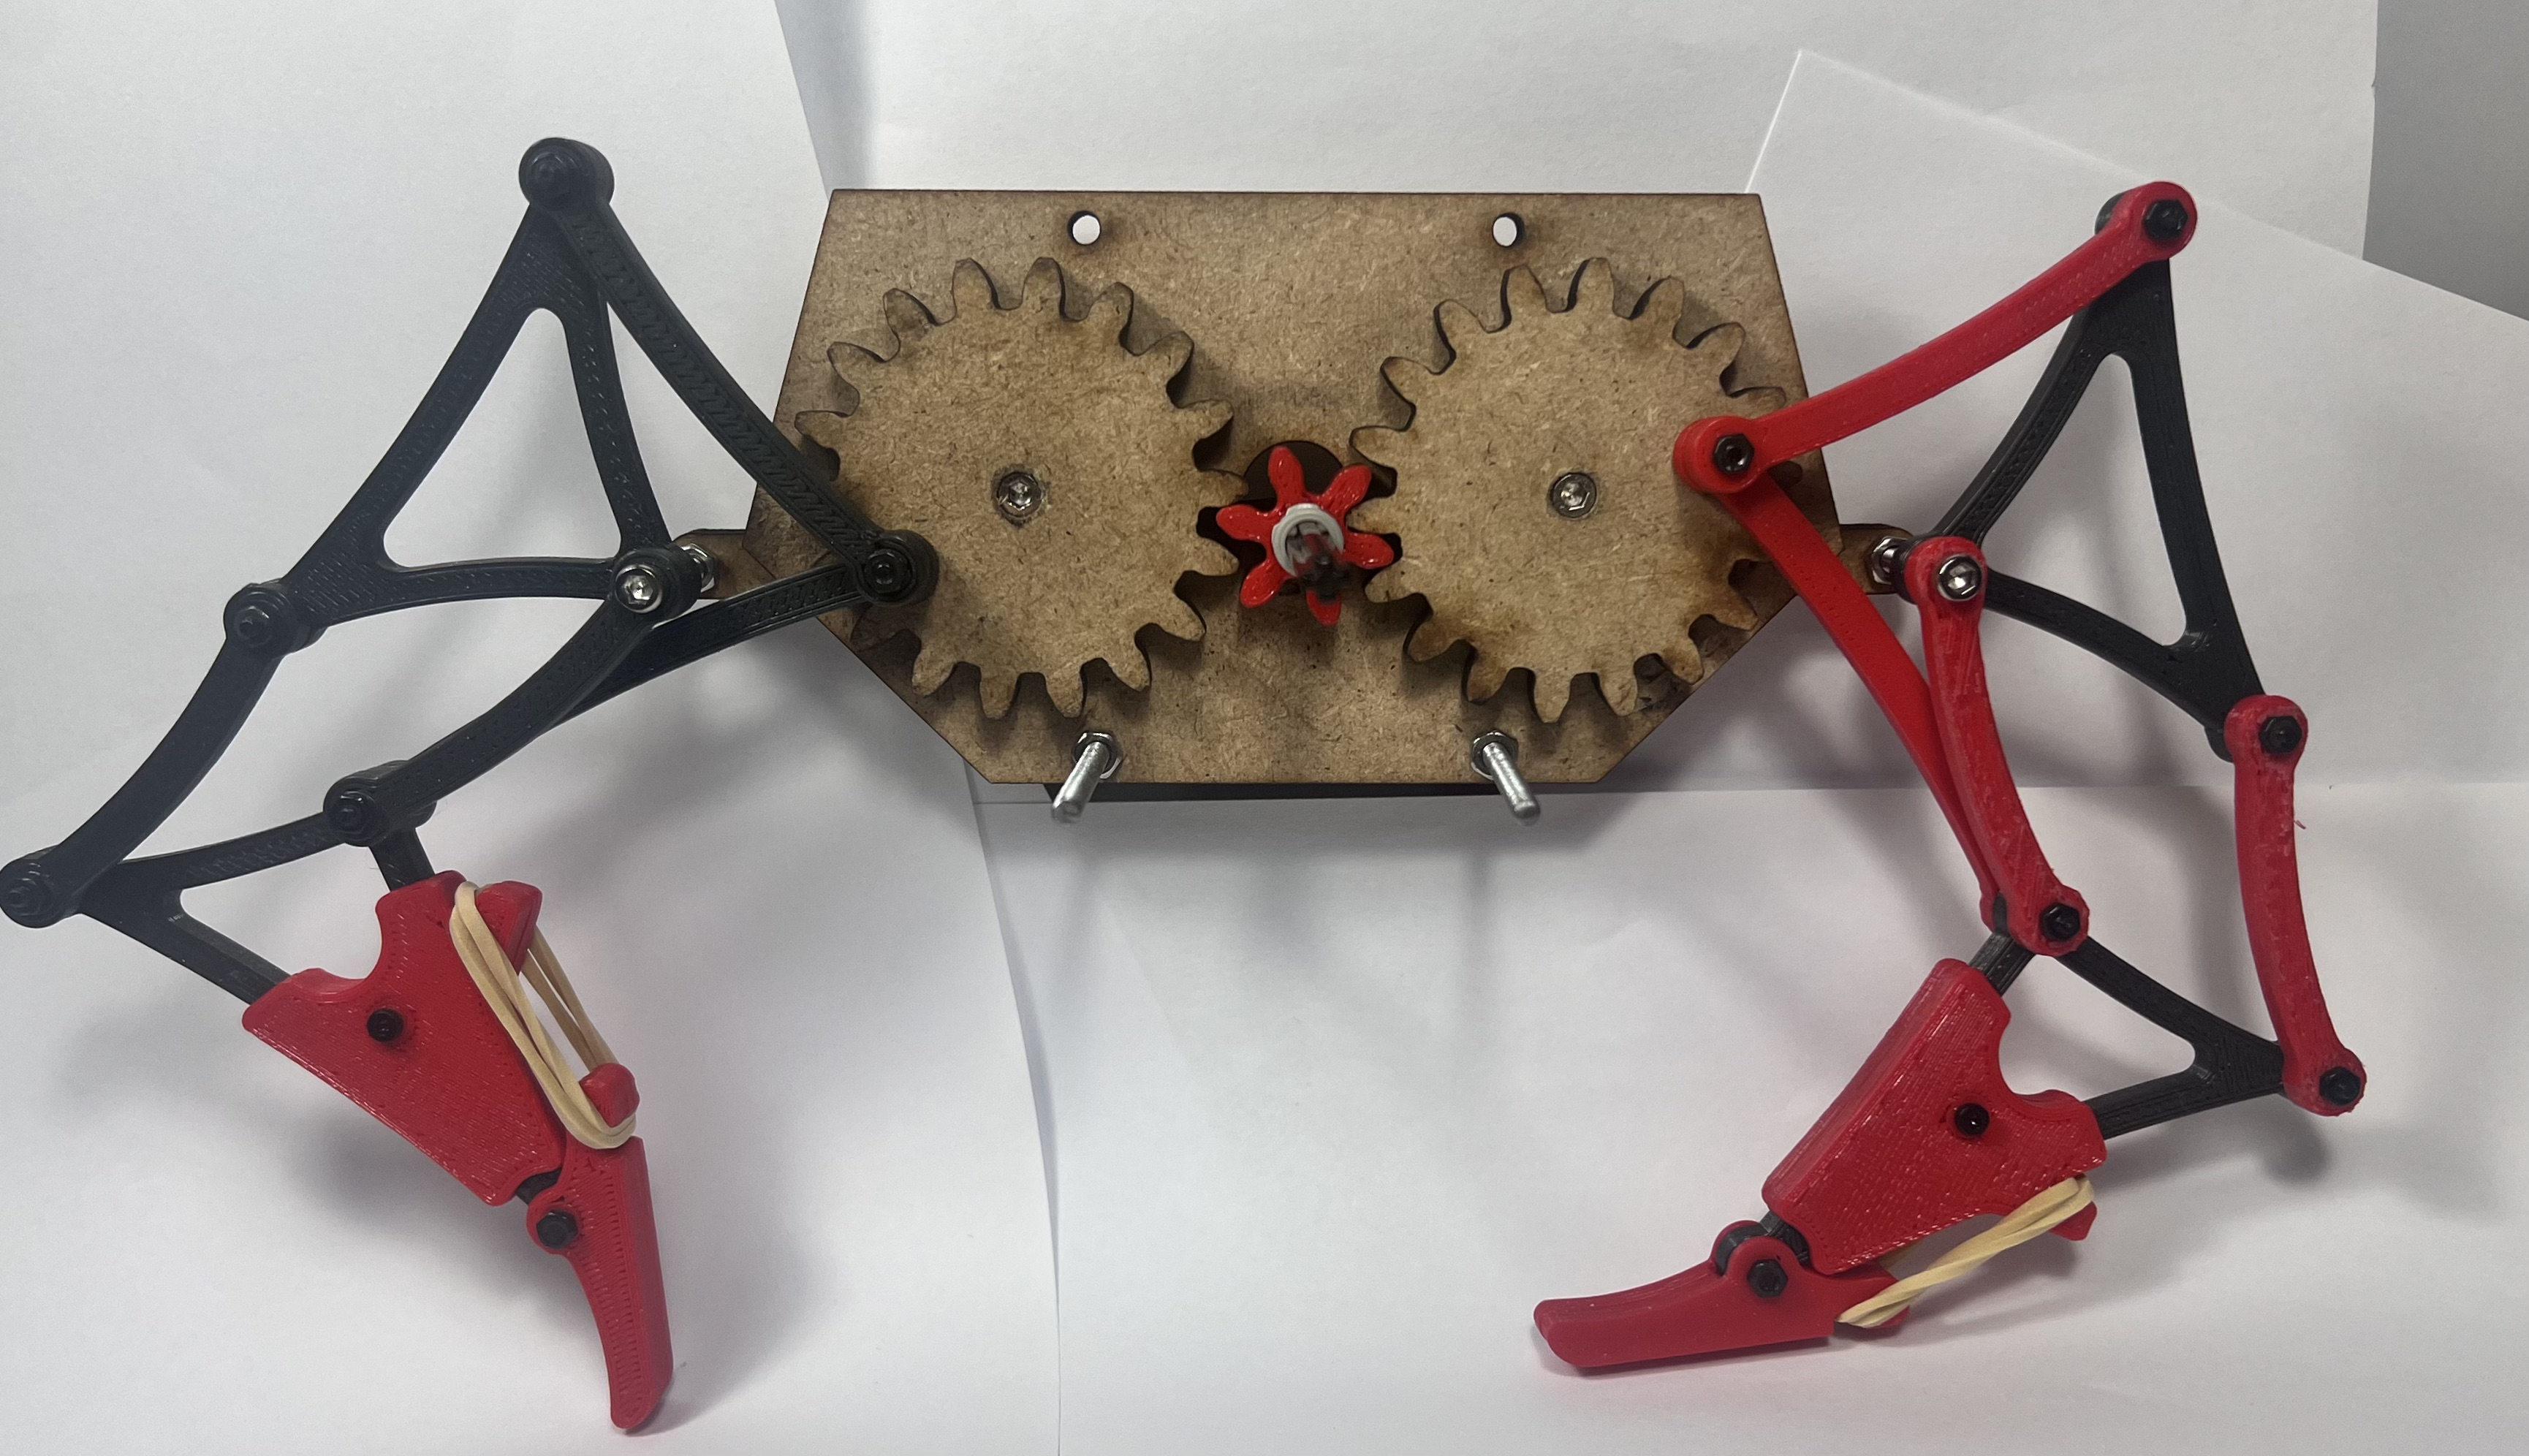
\includegraphics[width=1\linewidth]{images/LMA.jpeg}       
    \caption{Fully assembled leg mounting plate}
    \label{fig:leg_mount_plate}
\end{figure}
\subsubsection{Leg-mounting-plate}
The leg-mounting plate is attached to the base plate using a custom-designed L-bracket and serves as the mounting point for both the gears and legs. A central hole with a 12mm diameter is cut into the middle of the plate, accommodating the rotating central axle. On either side of this hole, two gears are mounted, which connect to the Theo Jansen linkages. These gears operate in a 1:3 ratio, effectively reducing the torque required from the motors. A 1:1 gear ratio was tested during development but was found to demand excessive torque, allowing movement only at the motors' maximum PWM setting. With the 1:3 gear ratio, movement—though slower—was achievable even at a PWM setting of 135.
\\ \\
A bracket is mounted on the back of the plate to secure one of the Theo Jansen joints in place. The primary design goal was to make the leg-mounting plate modular, enabling additional plates to be easily attached to either side. This was accomplished with two holes at the bottom of the plate where two 3mm metal rods can be inserted, and fastened with bolts, serving both as mounting points and alignment guides. The plate, was cut out of 6mm MDF, using a laser cutter. The thicker MDF was chosen because of the increased stress that these plates would incur. A fully assembled Leg-mounting-plate can be seen in figure: \ref{fig:leg_mount_plate}
\\
\subsubsection{Theo-jansen linkage}
The main mechanism of the robot is the Theo Jansen linkage, which acts as the legs. This type of linkage is a planar system with a single degree of freedom, meaning it can be driven by just one rotary input. When the central link is powered by a motor, it moves the rest of the connected links in a coordinated way, creating a smooth, walking motion that mimics a natural gait.
\\ \\
\begin{figure} [!htb]
    \centering
    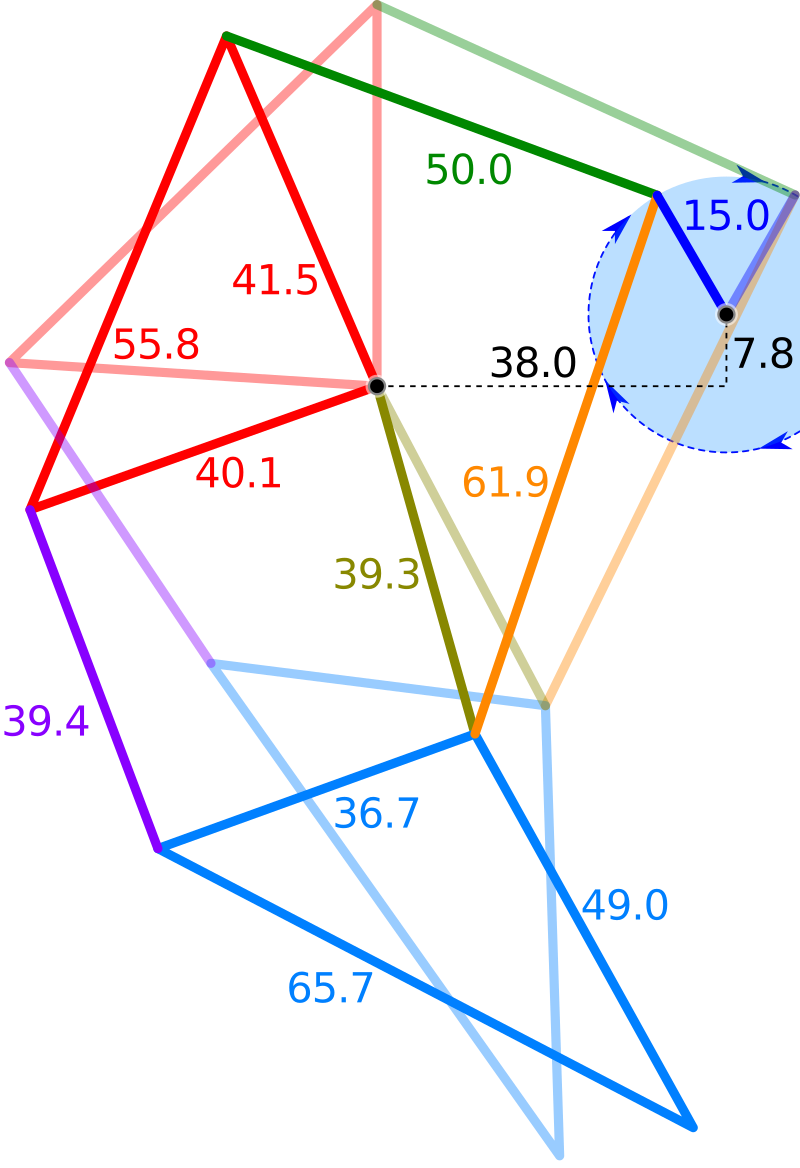
\includegraphics[width=1\linewidth]{images/Jansen's_Linkage.svg.png}
    \caption{Dimensions of the Theo Jansen linkage\cite{jansen2016strandbeest}}
    \label{fig:jansen_dimension}
\end{figure}
The linkage components are connected using revolute joints, which limit movement to rotation only. The leg design is based on common Theo Jansen dimensions (see figure: \ref{fig:jansen_dimension}. Two DC motors are used to drive the legs. Each motor is connected to a gear that turns the central linkage, powering the gear that turns the linkages. The gears, as mentioned above is set to a 1:3 gear ratio. The main joint of the linkage is attached to gear, while another joint is fixed in place using the bracket on the back of the Leg-mounting-plate. All other joints can move freely. Then, when the gear turns, the legs move in a natural gait. 
\\ \\
The main challenge in getting the Theo Jansen linkages to move smoothly is friction. Because of the downward pressure applied at each joint, significant resistance builds up, making motion less efficient. An additional source of friction comes from the contact between two linkages rubbing against each other within the joint. To reduce this effect, we experimented with different materials to determine which offered the lowest friction during movement. we tested two different materials for the linkage components: laser-cut MDF and 3D-printed PLA. The PLA parts resulted in noticeably less friction, allowing us to reduce the required PWM setting by 15 compared to the MDF version. We believe this improvement is because of the reduced surface contact area and smoother finish of the 3D-printed PLA components. \\
\subsubsection{Actuated feet}
In an attempt to increase stability and mobility on uneven terrain, the robot is equipped with actuated feet consisting of two components: a foot and a boot (figure: \ref{fig:feet}). These parts are designed as a clamshell that wraps around the lower leg segment and is secured using a single bolt and nut. A rubber band is attached from the heel of the foot to the boot, providing a passive return force that helps keep the foot in contact with the ground during motion. We found this setup to improve traction and energy transfer, allowing the robot to move on rougher surfaces and increasing the overall forward walking speed.
\begin{figure} [!htb]
    \centering
    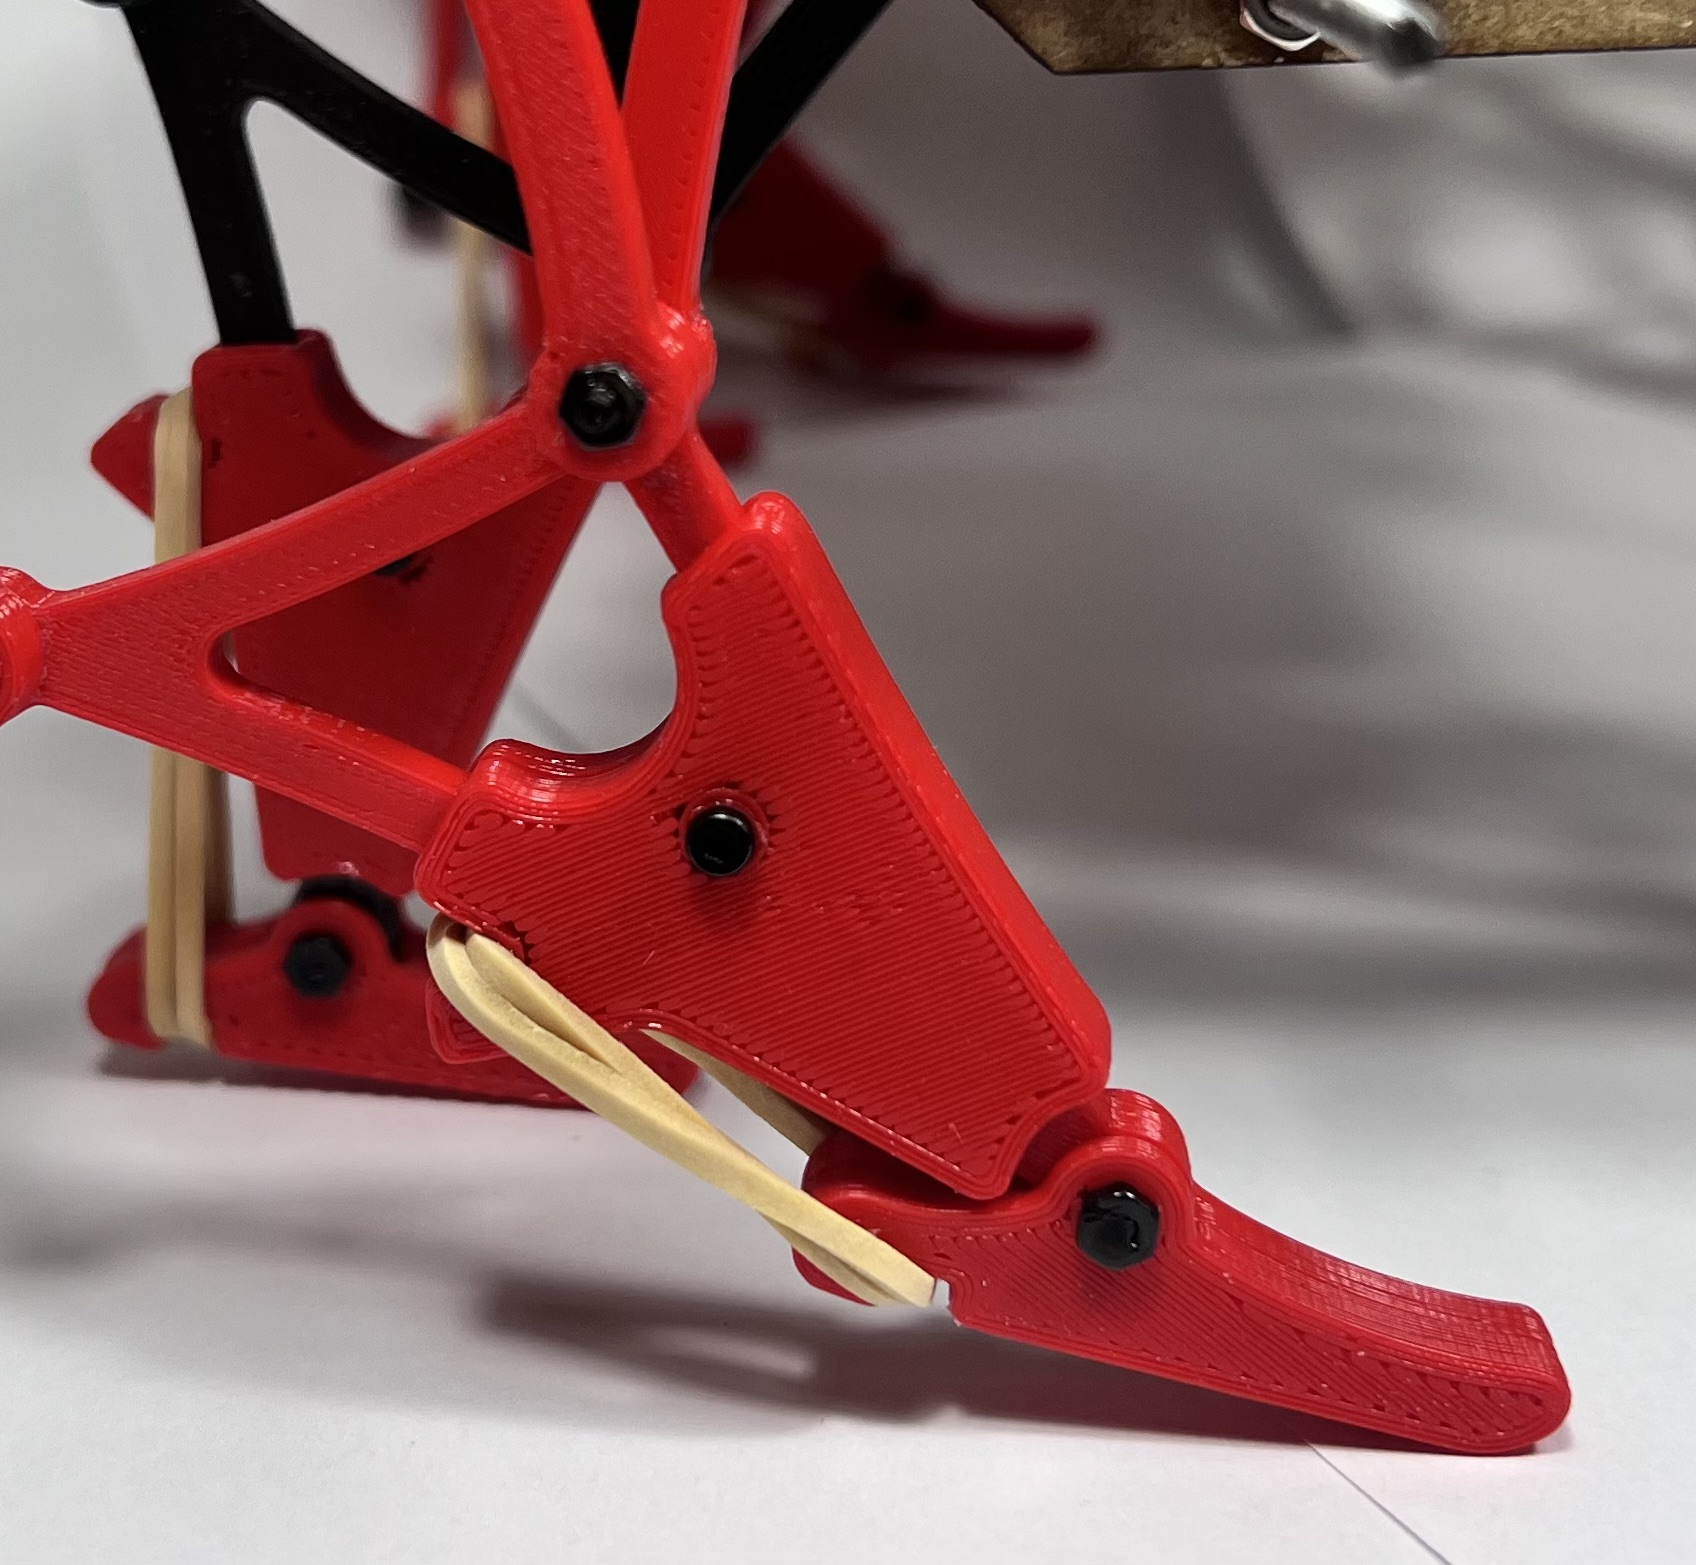
\includegraphics[width=1\linewidth]{images/Feet_assembly.jpeg}
    \caption{Acutated feet assembly}
    \label{fig:feet}
\end{figure}
\\ \\
One trade-off with this design is a reduction in backward walking speed, as the boot and foot are not symmetrical. Both parts are 3D-printed using PLA filament. To ensure a proper fit between the components, an inner wall tolerance of 0.25mm was used.
\subsection{Electronics}

\subsubsection{Microcontroller}
An Arduino Uno V3 is used as the microcontroller to manage all electronics of the robot. It distributes power from a 9V battery to the ultrasonic sensor, HM-10 Bluetooth module, and two DC motors. The onboard voltage regulator supplies 5V to components requiring lower voltage, such as the ultrasonic sensor and the HM-10 module. However, the motor shield provides the full 9V directly to the DC motors. The Arduino receives input from both the ultrasonic sensor and the Bluetooth module. Based on this data, it controls the movements of the robot by sending appropriate signals to the motor shield, which handles direction and speed control via PWM outputs. The entire circuit can be seen below in figure \ref{fig:Schematic}
\begin{figure} [!htb]
    \centering
    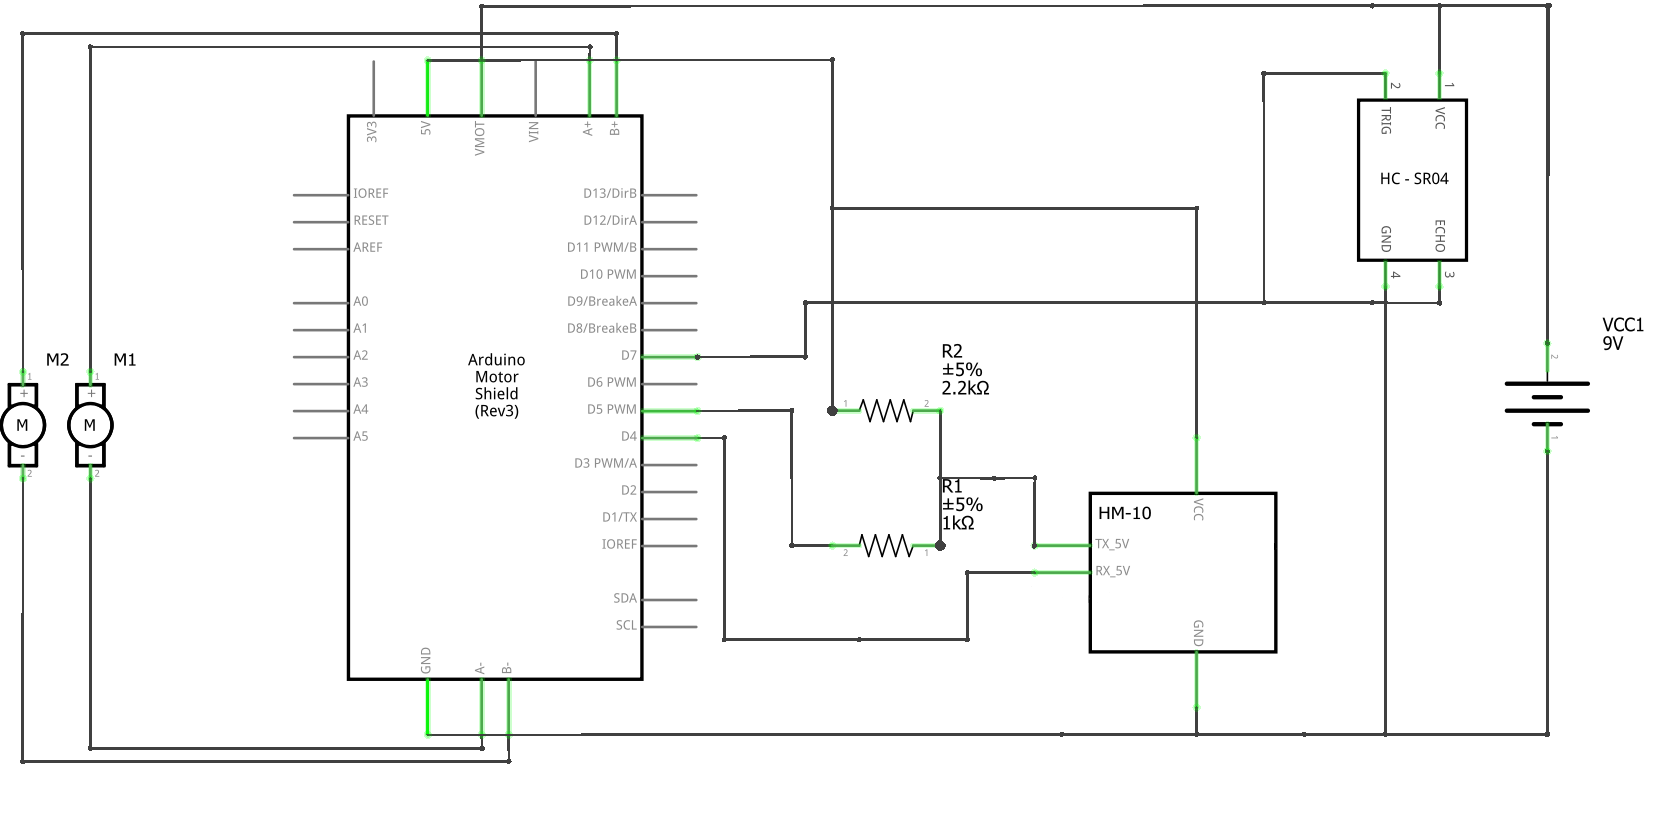
\includegraphics[width=1\linewidth]{images/Amandatory_exam_schem.png}
    \caption{Electronics schematic}
    \label{fig:Schematic}
\end{figure}
\subsubsection{Motor shield}
To simplify motor control and to help maintain a clean layout, a motor shield was used. The shield is based on the L298P dual H-bridge driver and mounts directly onto the Arduino, removing the need for additional wiring between the Arduino and a separate motor driver module. The L298P-based shield enables control of both the direction and speed of the motors. Directional control is achieved without manually constructing an H-bridge circuit, while speed is regulated using PWM (Pulse Width Modulation). This level of control was useful during testing of the robot, as it allowed us to evaluate how changes in mechanical design affected the required PWM values for minimal movement.
\\
\subsubsection{Ultra Sonic sensor (HC-SR04)}
To handle obstacle detection and prevent the robot from steering into walls, an ultrasonic sensor is used to detect nearby objects. The sensor is mounted to the baseplate using a custom bracket to ensure a forward-facing orientation. Depending on the model, the HC-SR04 ultrasonic sensor can have either three or four pins. In this implementation, a 3-pin version is used, which includes GND, VCC, and Signal. VCC and GND are connected to the Arduino’s 5V power rail and ground, respectively, while the Signal pin is connected to digital pin 7 on the Arduino. The ultrasonic sensor works by sending out a short burst of sound and measuring the time it takes for the echo to return. This data is then used to calculate the distance. 
\\
\subsubsection{Bluetooth interface (HM-10)}
One of the goals for this project was to be able to remote control the robot from a smartphone or other device, as such a communication device was needed to communication between the Arduino and external devices, a Bluetooth module was selected. After evaluating two common options, the HC-06 and the HM-10 we elected for the HM-10 due to its compatibility with IOS devices and support for Bluetooth Low Energy (BLE), which offers lower power consumption. The HM-10 module features four pins: VCC, GND, TXD (transmit), and RXD (receive). VCC and GND are connected to the Arduino’s 5V power rail and ground, respectively. Serial communication is handled via the TXD and RXD pins, which are connected to digital pins 4 and 5 on the Arduino.
\\ \\
Since the HM-10 operates on 3.3V logic levels, a voltage divider is used on the Arduino’s TX line to reduce the 5V signal to 3.3V. The RXD line from the module, which sends data to the Arduino, can be read directly without level shifting, as 3.3V is sufficient for a logic high on Arduino boards. The module recives data from a smartphone app, which controls the direction and speed of the robot.
\\
\subsubsection{DC-motor}
To drive the main axles on either side of the robot, DC motors were selected. Stepper and servo motors were considered, but not chosen, as the application did not need precision positioning. Instead, the focus was on sufficient torque to overcome friction. A lower RPM motor was chosen, rated at approximately 60 RPM. This slower motor provides higher torque. Alternatively, we could have used a higher RPM motor, though it would have been necessary to increase the gear ratio to achieve similar torque output. The DC motors are connected to the Arduino via the motor shield, allowing for both directional and speed control. Speed is regulated using PWM signals, enabling the system to adjust power to the motors.
\\
\subsubsection{Power}
To power both the Arduino and the DC motors, a 9V battery was used. This choice was made to provide higher voltage to the motors, improving their performance compared to lower-voltage alternatives. However, a drawback of the 9V battery is its capacity under load, resulting in frequent battery replacements during extended testing. An alternative setup using four 1.2V rechargeable batteries was tested, but ultimately rejected. This setup resulted in noticeably reduced motor performance and introduced a lot of additional weight. Both of those compounding factors led continuing to use of the 9V battery.
\\
\subsection{Software/Firmware}
This project involves two software components: the Arduino code, which controls the robot and reads data from the Bluetooth and ultrasonic sensors; and the IOS app, which sends signals to the Bluetooth module. Since app development is outside the scope of the course, only a brief overview of the UI and implementation will be provided. \\
\subsubsection{Arduino firmware}
The primary functions of the Arduino software is motor control, Bluetooth communication, and obstacle detection. Motor control is implemented via the motor shield, which enables control of motor direction, braking, and speed using PWM signals. Each motor is controlled using three pins: one for direction, one for braking, and one for speed (PWM). The direction and brake pins are digital and can be set to either HIGH or LOW to enable, disable, or reverse motor rotation. The speed pin uses PWM and accepts analog values between 0 and 255, enabling fine motor control. Appendix \ref{arduino_code} for source code
\\ \\
Commands are received via the HM-10 Bluetooth module. Upon receiving a command, the Arduino updates the relevant control pins for each motor accordingly. The system supports five directional commands: forward, backward, left, right, and stop. In addition to directional control, the Arduino can process speed commands that adjust the PWM output by increments of ±10, ±25 and ±50.
\\ \\
Obstacle detection is handled using the HC-SR04 ultrasonic sensor, which measures the distance to objects in front of the robot. If the detected distance falls below a defined threshold, the Arduino engages the motor brakes to prevent collisions. In this state, only speed, turn or reverse commands are accepted, ensuring that the robot avoids driving into obstacles.
\\
\subsubsection{IOS-app}
\begin{figure}
    \centering
    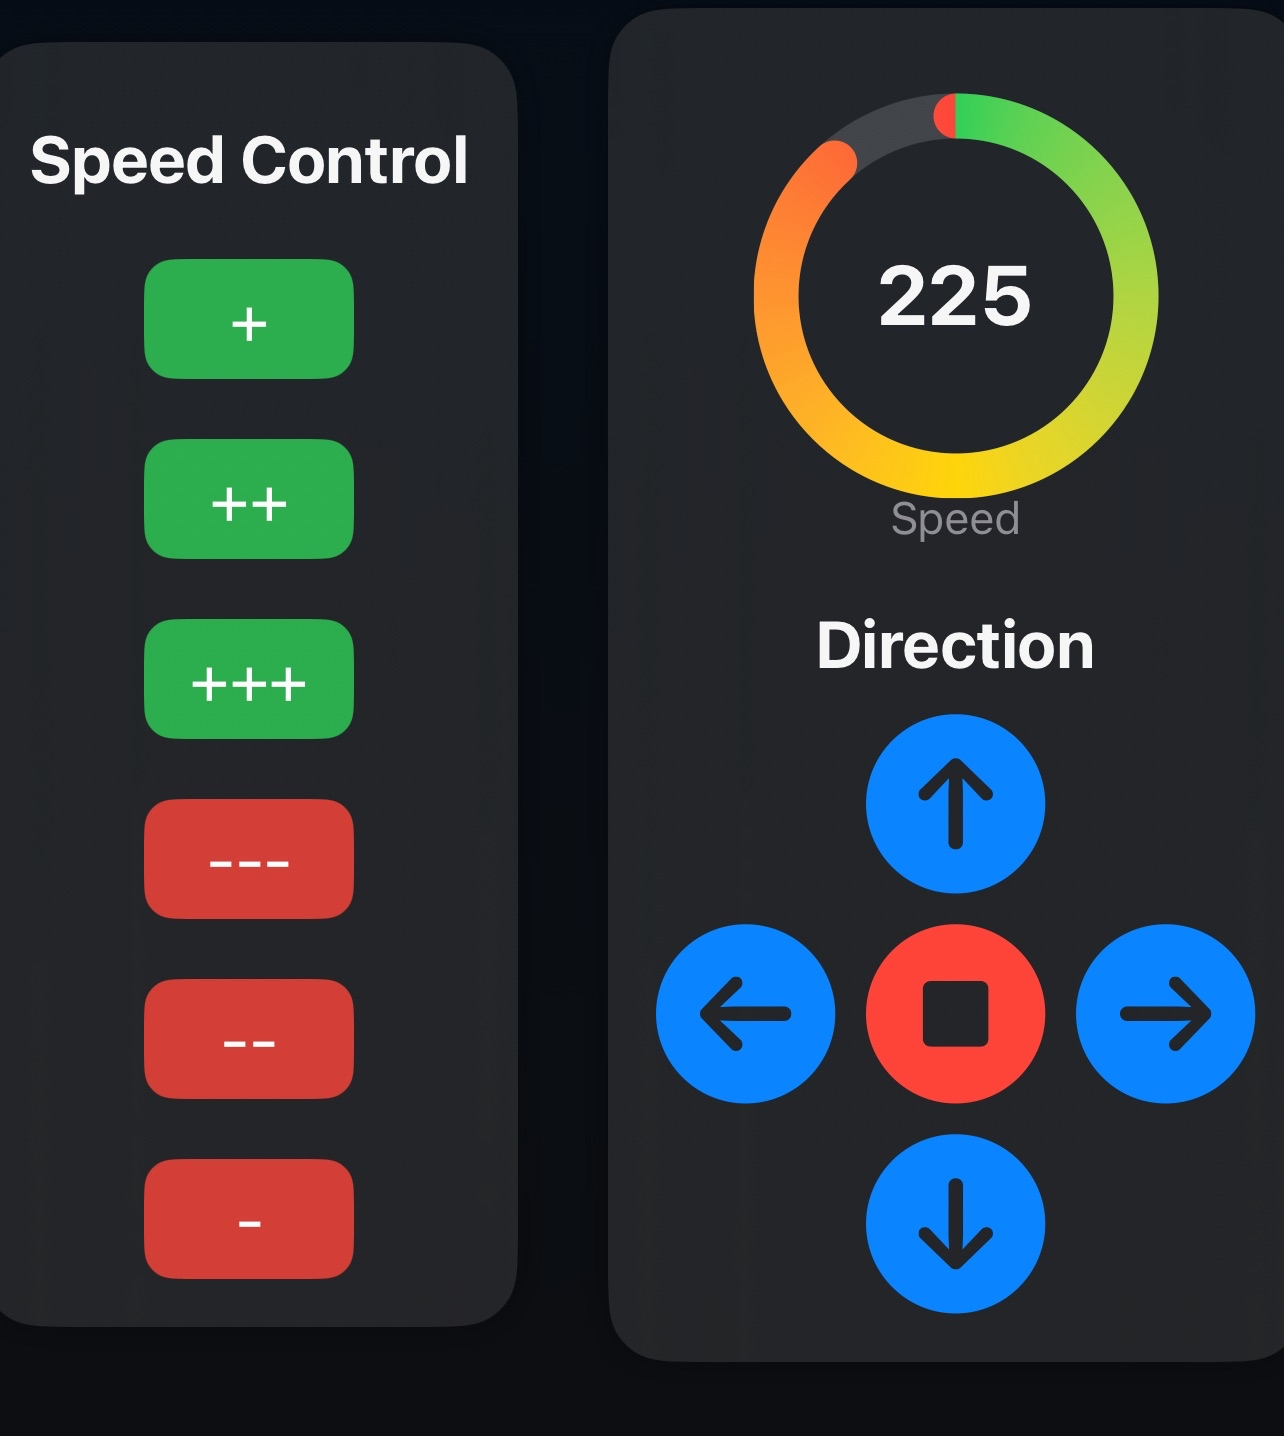
\includegraphics[width=1\linewidth]{images/IOS_app_interface.png}
    \caption{Interface of the app, with a PWM setting at 225}
    \label{fig:app_interface}
\end{figure}
The IOS app (see appendix: \ref{swift_code}, for source code), developed in Swift, connects to the HM-10 Bluetooth module on startup and automatically attempts to reconnect if the connection is lost. It features five directional buttons (forward, backward, left, right, stop) and six speed adjustment buttons (±10, ±25, ±50). A speedometer displays the current PWM value. When a button is pressed, the app sends the corresponding command to the Arduino via Bluetooth. The app interface is shown in Figure \ref{fig:app_interface}.